\section[COMPONENTES, FRAMEWORKS E FERRAMENTAS]{COMPONENTES, \emph{FRAMEWORKS} E FERRAMENTAS}
Neste item serão analisados os components, \emph{frameworks} e ferramentas que foram selecionadas para construção do software. 
Este software será um serviço disponibilizado via \emph{web}, sendo assim, estas tecnologias são próprias para este fim. 

\subsection{APLICAÇÕES WEB COM \emph{ANGULAJS}}
\label{angularjs}
O \emph{AngularJS} é um \emph{framework} de aplicação \emph{web}. 
Ele foi projetado especificamente para rodar em \emph{browsers} que suportam \emph{HTML 5}.
Ele também é adequado a criação de aplicações \emph{web} que rodam em \emph{smartphones}. 
É um \emph{framework} bastante completo e rico para sua finalidade. 
A referência \citeonline{Branas2014} é um guia introdutório conciso no assunto.
 Segundo \citeonline{Freeman2014}, outro guia no assunto, o \emph{AngularJS} se baseia no padrão de projeto \emph{Model-View-Controller (MVC)} e sua enfase é em permitir a criação de aplicações: extensíveis, manuteníveis, testáveis e padronizadas. 
A Figura \ref{angularjs_mvc} mostra uma representação de uma aplicação fazendo uso do \emph{AngularJS}.

\begin{figure}[ht]
	\centering
	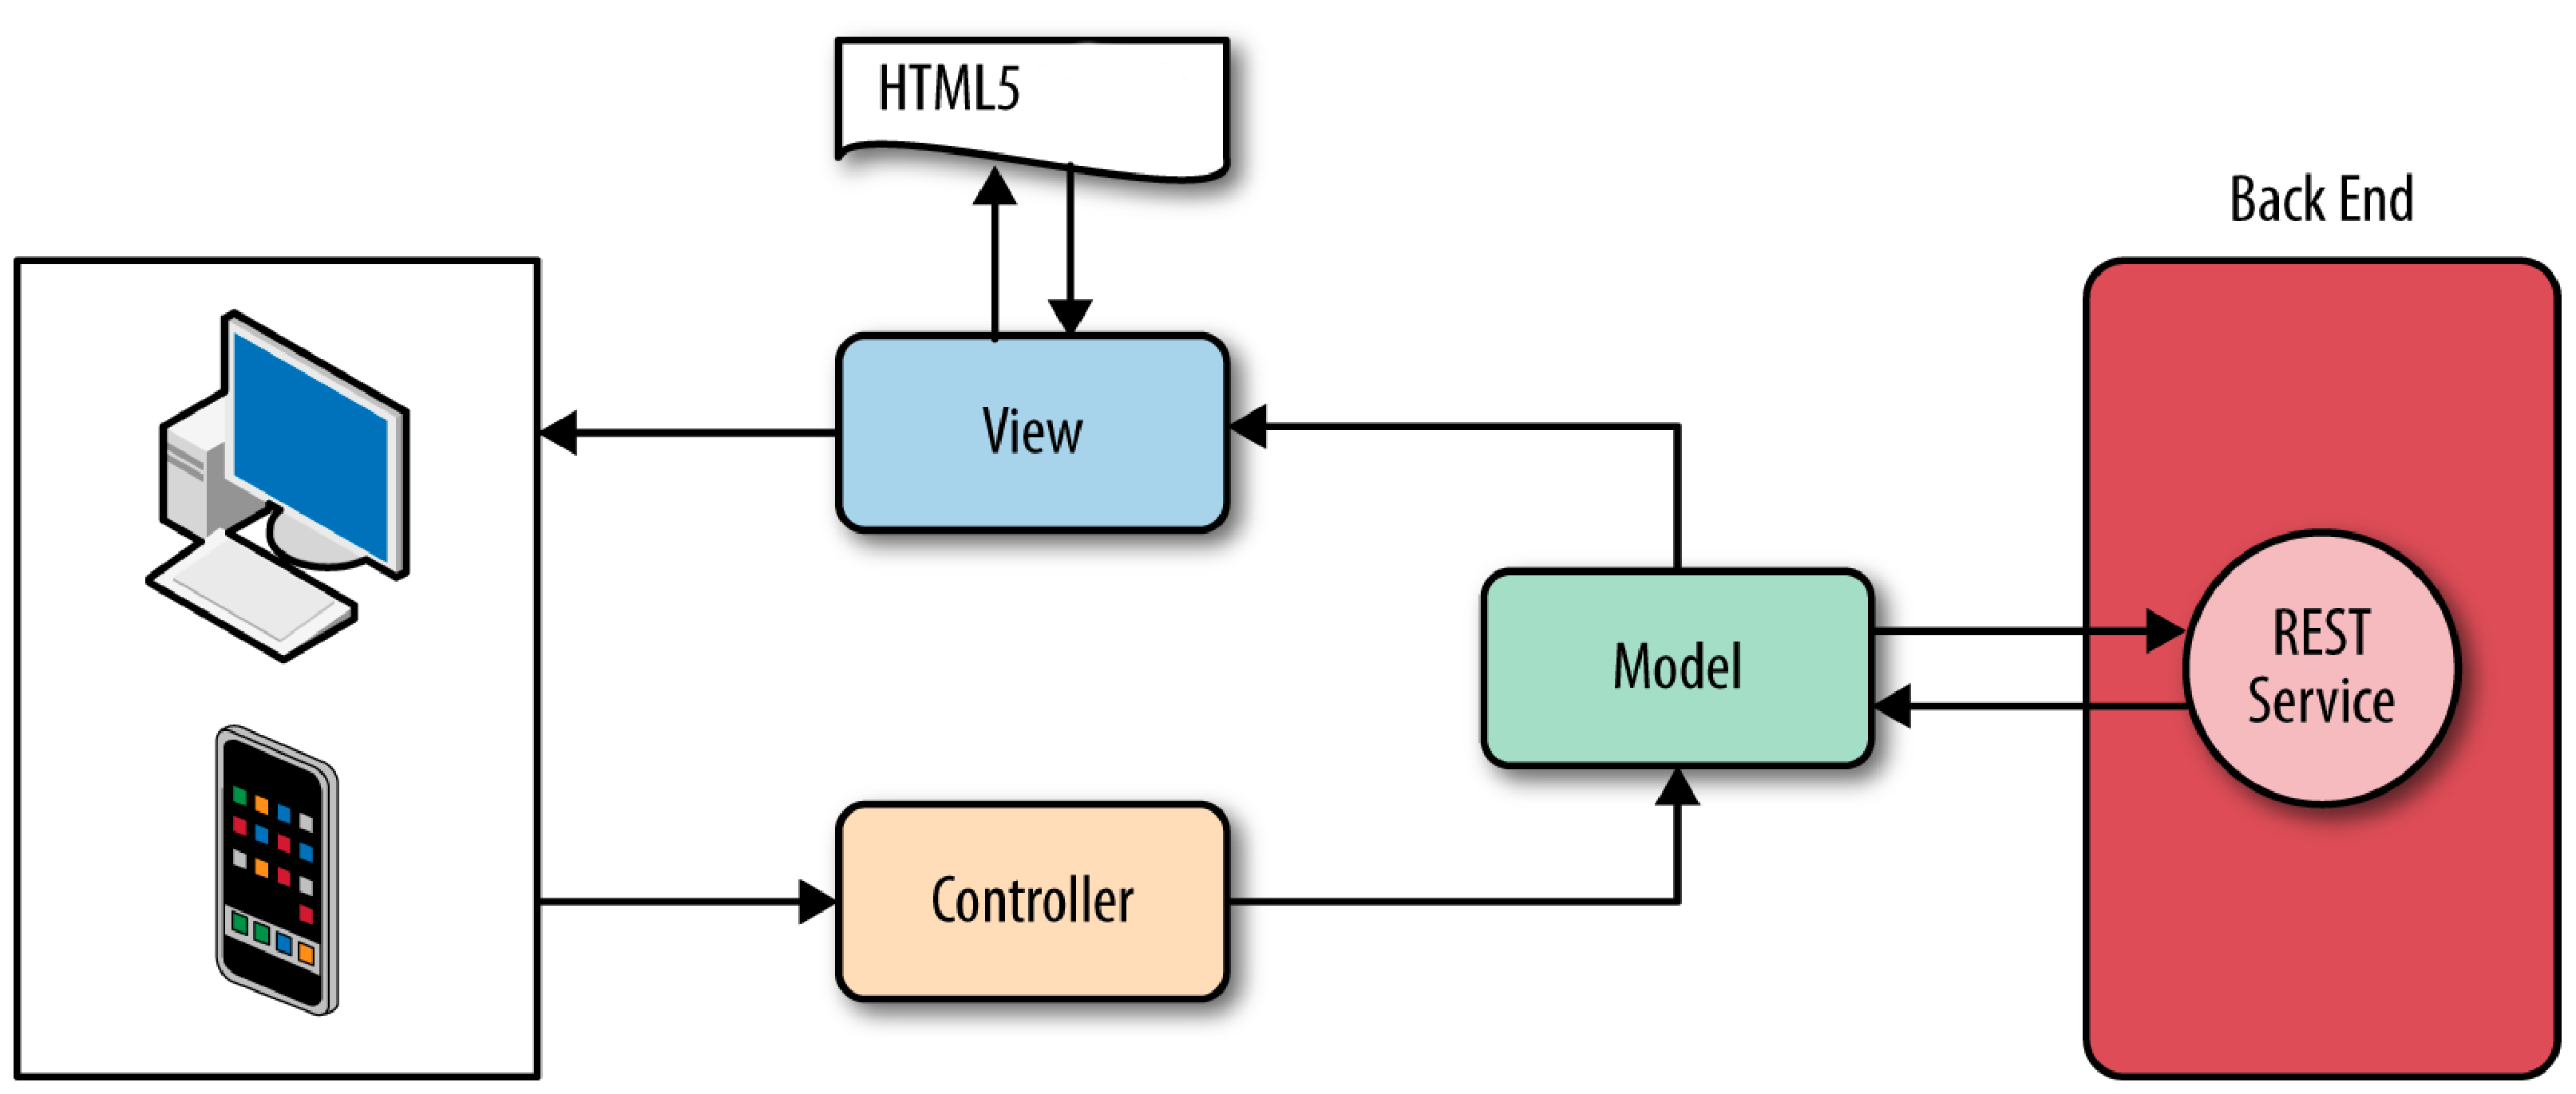
\includegraphics[width=14cm]{figuras/angulajs_mvc.eps}
	\caption{Diagrama de uma aplicação \emph{MVC} usando \emph{AngularJS}.}
	\label{angularjs_mvc}
	\footnotesize Fonte: \citeonline{Williamson2015}.
\end{figure}

Segundo \citeonline{Williamson2015}, a Figura \ref{angularjs_mvc} mostra o diagrama de uma aplicação \emph{AngularJS} e os componentes \emph{MVC}.  Uma vez que a aplicação é lançada, os componentes \emph{model, view} e \emph{controller}, juntamente com todos os documentos \emph{HTML} são carregados no \emph{desktop} ou \emph{smartphone} do usuário e rodam completamente num destes hardwares.  A aplicação \emph{AngularJS} conversa com o \emph{backend} via o protocolo \emph{http}.  O \emph{backend} é um servidor \emph{web} que mantém chamadas \emph{REST} (explicado na seção \ref{servicos_rest}), sendo responsável pela execução da lógica e de processos de negócio.  
Outra característica bastante apreciada pelos desenvolvedores que usam \emph{AngularJS}, é a possibilidade de criar \emph{single-page aplications (SPA)}. 
\emph{SPAs} são aplicações que tem uma página \emph{HTML} de entrada. 
Esta página tem seu conteúdo dinamicamente adicionado e removido da mesma.
Esta abordagem permite criar aplicações bastante interativas, lembrando mesmo, aplicações \emph{desktop} escritas em linguagens como \emph{Visual Basic} e \emph{Delphi}.

\subsection{ORGANIZAÇÃO DE PROJETOS WEB COM \emph{ANGULAR-SEED}}
\label{angular_seed}

O \emph{angular-seed}, é um \emph{template} para projetos \emph{web} que utilizam o \emph{AngularJS}. 
Ele facilita bastante o processo de configuração e padronização do projeto. 
Ele cria um \emph{layout} de diretórios padronizado, pré-configura as ferramentas de \emph{build} e também já pré-configura o ambiente de testes unitários \emph{web/javascript} usando a ferramenta \emph{JASMINE}. 
Mais informações sobre o \emph{angular-seed} em \citeonline{Google2015b}.

A Figura \ref{seed} mostra o \emph{layout} inicial de diretórios que a ferramenta gera após ser clonada do \emph{Github}.

\begin{figure}[ht]
	\centering
	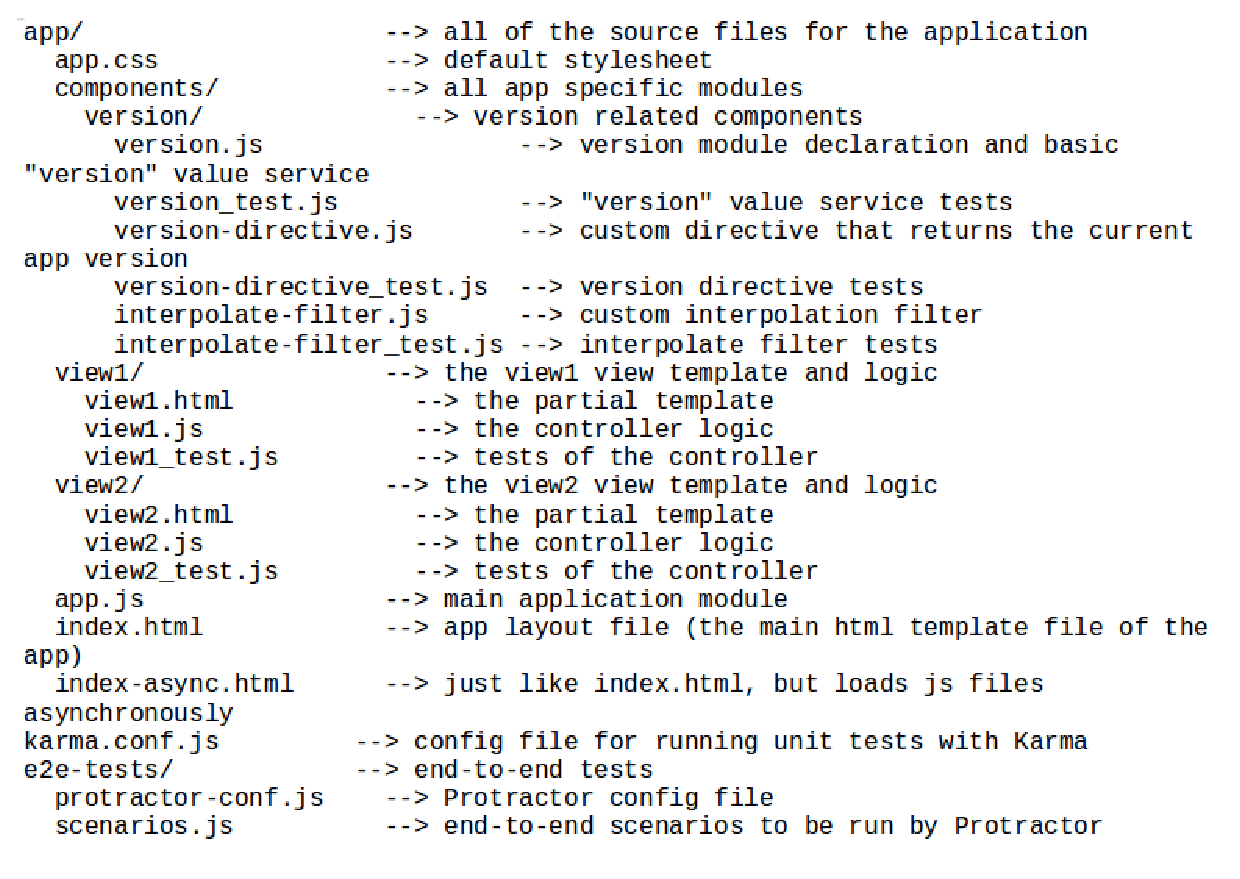
\includegraphics[width=14cm]{figuras/seed.eps}
	\caption{Layout original de um projeto baseado em \emph{angular-seed}. Fonte: \citeonline{Google2015b}.}
	\label{seed}
\end{figure}

Antes de começar a usar o \emph{angular-seed} é necessário instalar o ambiente de execução \emph{Javascript Node.JS}. 
Este ambiente é utilizado para execução de testes e construção de \emph{builds}. Para uma introdução ao \emph{Node.JS} veja \citeonline{Syed2014}.
\subsection{SOLUÇÃO DE DESIGN WEB COM \emph{ANGULAR-MATERIAL}}
\label{angular_material}

Os usuários profissionais da área de saúde, dificilmente se interessariam por um software complexo sem uma interface atraente e amigável.
Uma solução para minimizar este problema é a adoção da  biblioteca \emph{angular-material}. 
Esta biblioteca, como indicado pelo seu nome, é construída com o \emph{AngularJS}. 
Ela disponibiliza serviços e diretivas que podem ser usados para construir a interface gráfica da aplicação. 
Diretivas são componentes que podem ser inseridos diretamente no código HTML da aplicação, dando a aparência de estender a própria HTML. 
Por exemplo, a diretiva \emph{md-button} da biblioteca é um tipo de botão que não é próprio do HTML. 
Outros exemplos de diretivas são: caixas de diálogos, barras de ferramentas, barras de progresso, grades, \emph{tooltip}, etc. 
Esta biblioteca é baseada na especificação \emph{Material Design} criada pela empresa \emph{Google}. 
A especificação discorre sobre padrões de designe gráfico e interação com usuário e é baseada no princípio da metáfora de materiais. 
Esta metáfora é uma teoria unificada de um espaço racionalizado e sistemas de movimento, isto segundo \citeonline{Google2015a}. 
Outra vantagem da biblioteca é que ela é projetada para se adaptar a diferentes tipos de dispositivos com telas de tamanhos diferentes.
Veja um exemplo de aplicação que usa \emph{angular-material} na Figura~\ref{material_1}.


\begin{figure}[ht]
	\centering
	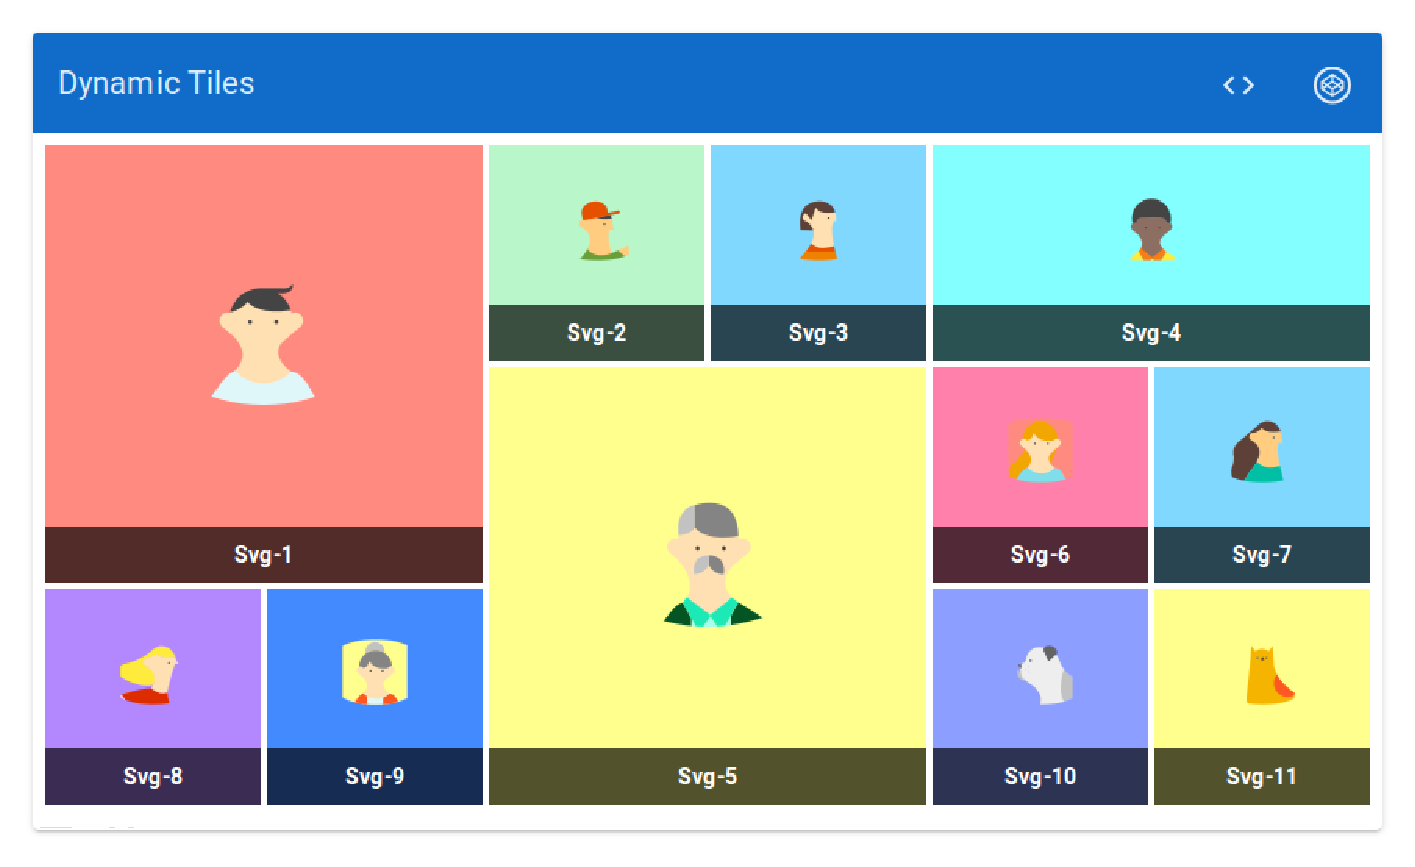
\includegraphics[width=14cm]{figuras/material.eps}
	\caption{Exemplo de aplicação que utiliza \emph{angular-material}. Fonte: \citeonline{Google2015c}.}
	\label{material_1}
\end{figure}



\subsection{GRÁFICOS E ANIMAÇÕES 3D NA \emph{WEB} COM \emph{THREEJS}} 
\label{threejs_sec}
Os \emph{browsers} modernos hoje, inclusive os dos \emph{smartphones}, suportam o novo padrão \emph{WebGL}. 
Este é um padrão \emph{web} multi-plataforma de \emph{API} de baixo nível para gráficos 3D, expostos através de \emph{HTML}. 
Este padrão suporta o acesso da \emph{API} usando-se a linguagem \emph{GLSL}. 
Uma vantagem desta API é que ela suporta nativamente \emph{GPUs} disponibilizadas pelo hardware que está executando o cliente \emph{web}. 
Isto torna possível até mesmo a criação de jogos de alta definição em 3D que rodam no \emph{browser} \cite{Matsuda2013}.

O problema com a \emph{WebGL} é que, como dito anteriormente, a \emph{API} é de baixo nível. 
No contexto de computação gráfica, isto significa que ela fornece primitivas básicas para modelagem 3D e outras opções de otimização do hardware.
Para resolver este problema bibliotecas em \emph{javascript} foram desenvolvidas, disponibilizando funções e objetos de alto nível, como cilindros, planos, esferas, animações, entre outros. 
Uma opção é o \emph{ThreeJS}, descrito em \citeonline{Dirksen2015}. 
Esta biblioteca apresenta um grande número de funcionalidades e é possível encontrar aplicações e jogos em 3D de nível profissional. 
Um exemplo de animação renderizada que utiliza \emph{ThreeJS} é mostrada na Figura \ref{evil_eye}.
Mais exemplos podem ser vistos no site \emph{threejs.org}.



\begin{figure}[H]
	\centering
	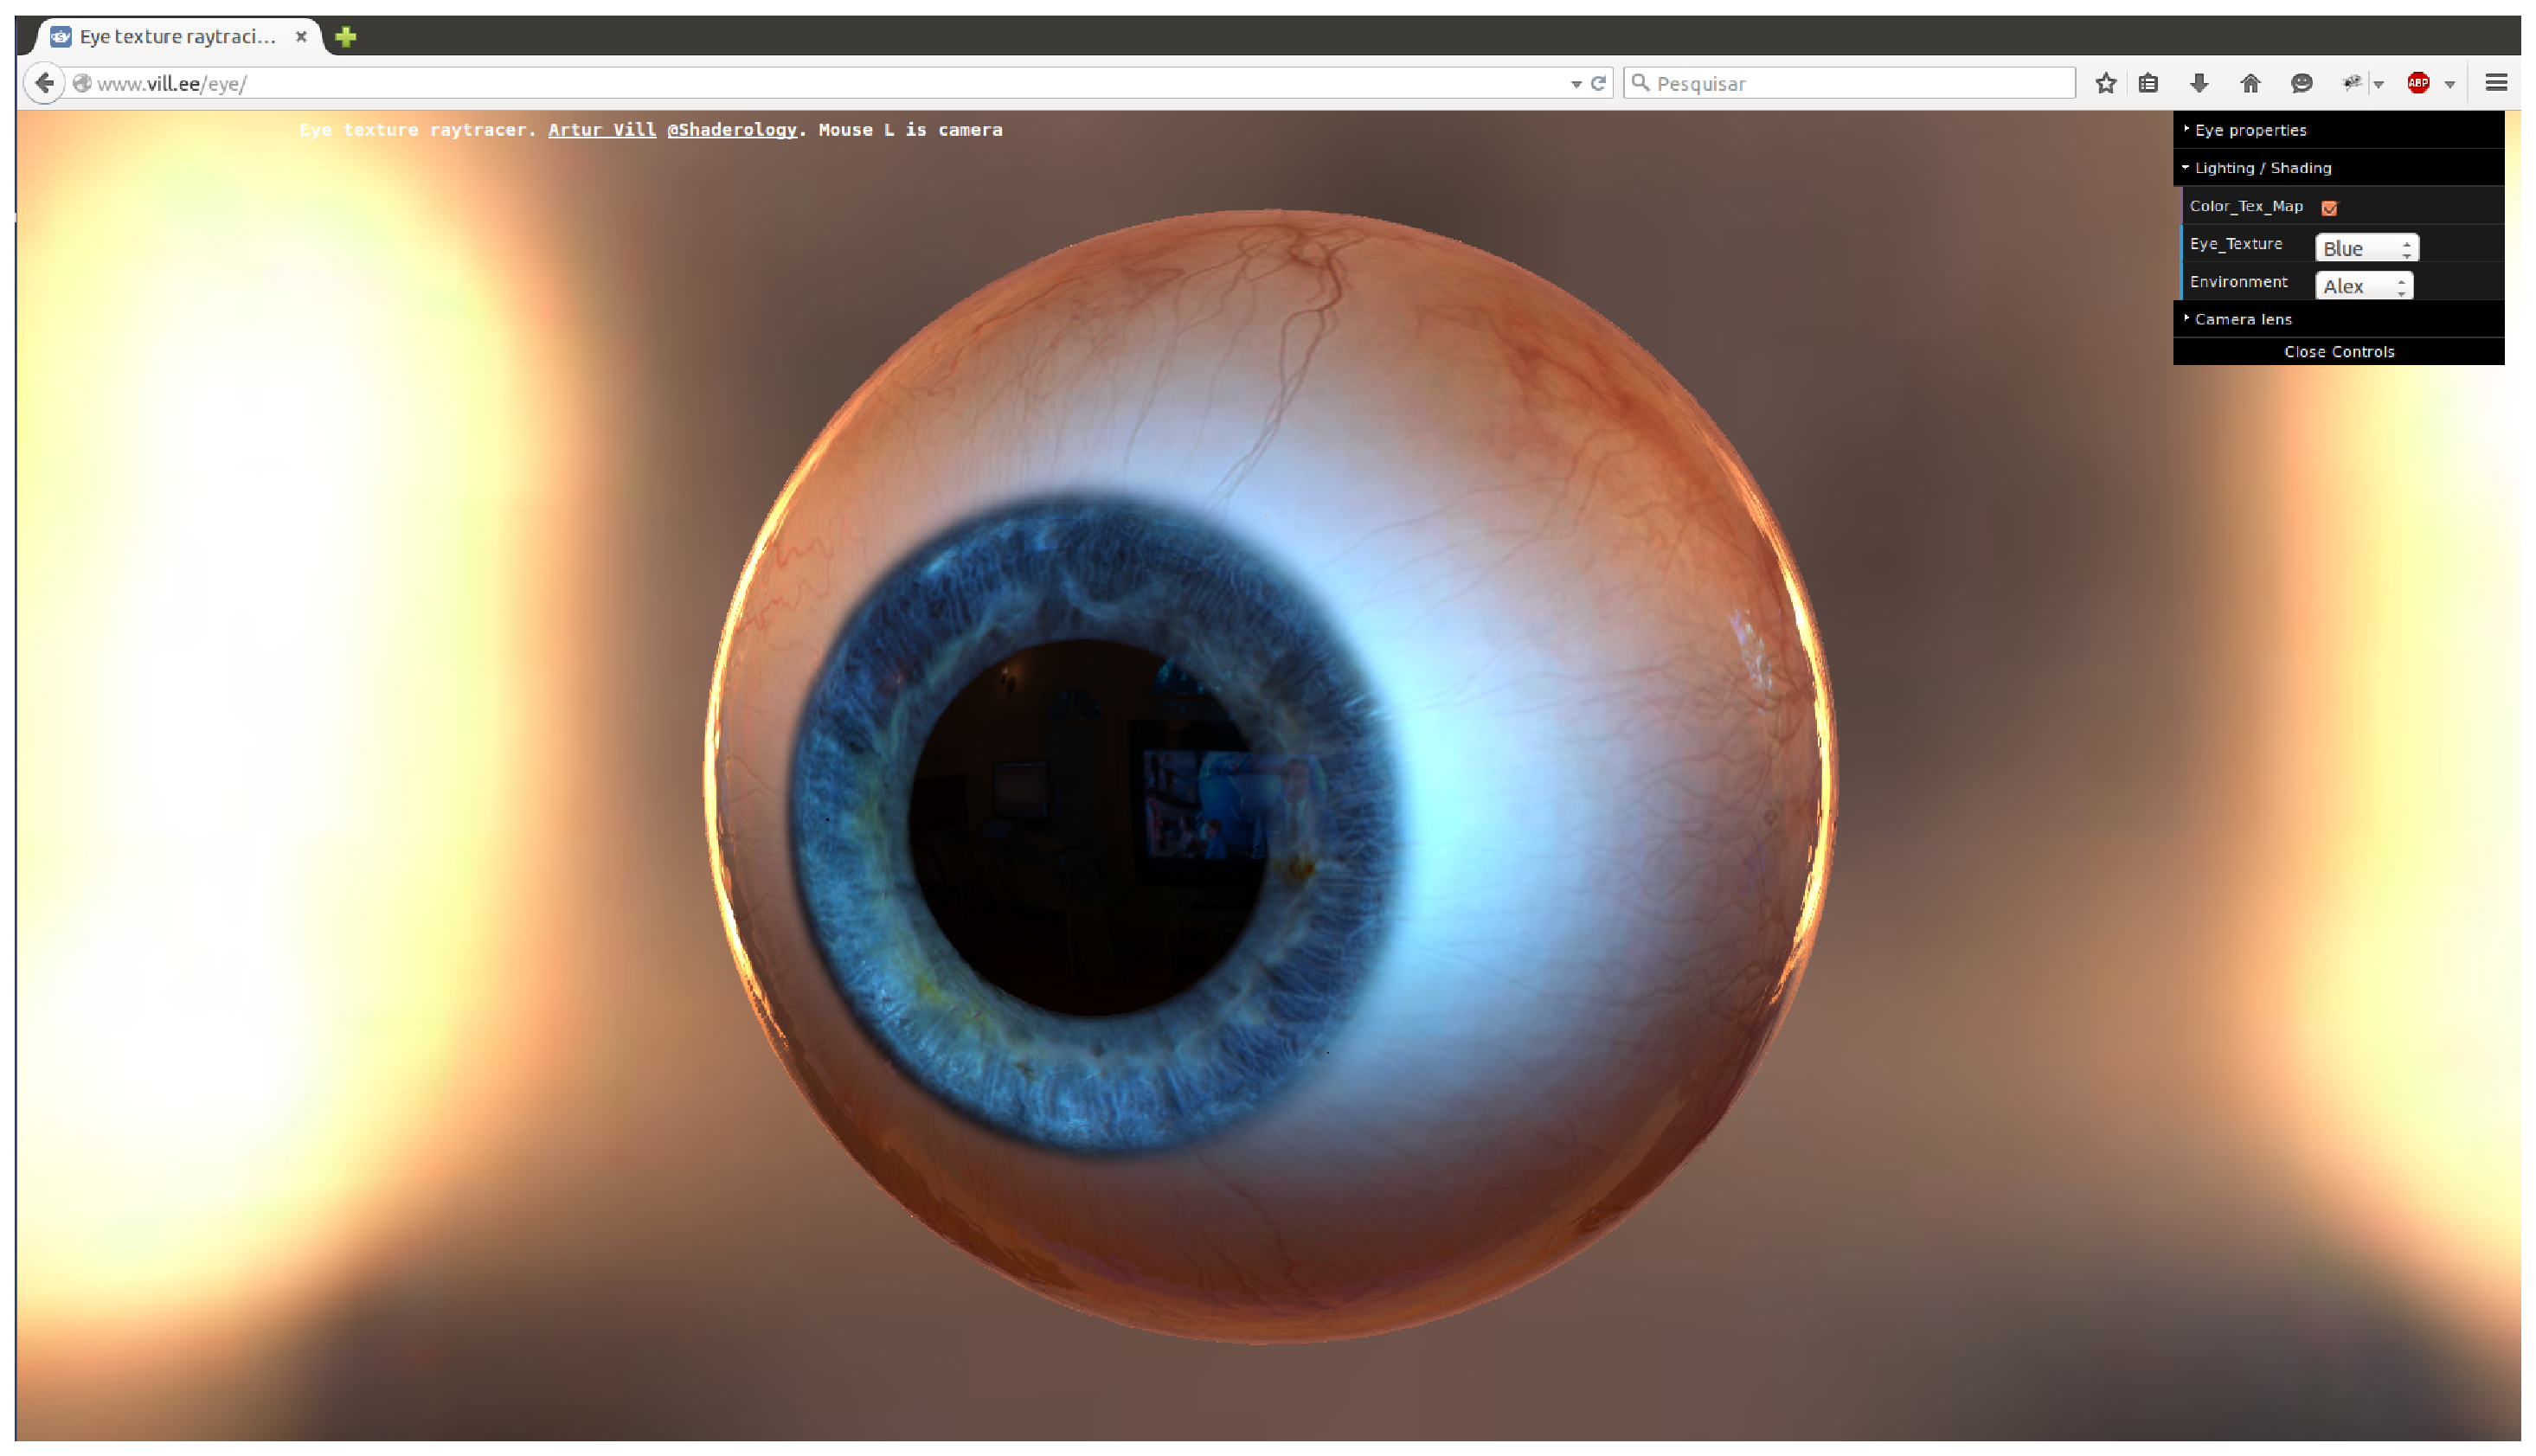
\includegraphics[width=14cm]{figuras/evil_eye.eps}
	\caption{Exemplo de aplicação que utiliza \emph{ThreeJS}.}
	\label{evil_eye}
	\footnotesize Fonte: \url{http://www.vill.ee/eye/}.
\end{figure}


\subsection{SERVIÇOS REST COM \emph{FLASK}}
\label{servicos_rest}

O \emph{Representational State Transfer (REST)} foi primeiramente descrito por \citeonline{Fielding2000}. 
Ele é definido como um estilo arquitetural de sistemas hipermídia e tem as seguintes características descritas por \citeonline{Grinberg2014}:

\begin{enumerate}
	\item Cliente-Servidor. Há uma separação clara entre quem consome, cliente, e quem serve e executa a lógica de negócio, servidor;
	\item \emph{Stateless}. O cliente precisa incluir nas suas requisições, todas as informações necessárias para o servidor processar o pedido. O servidor não armazena informações de estado do cliente entre as requisições deste;
	\item Interface Uniforme. O protocolo que os clientes usam para acessar o servidor precisa ser consistente, bem definido e padronizado. O protocolo comumente usado por serviços \emph{REST} é o \emph{HTTP};
	\item Sistema em Camadas. Servidores \emph{proxy}, \emph{caches} ou \emph{gateways}, podem ser inseridos entre clientes e servidores quando necessários, para melhorar a performance, confiabilidade e escalabilidade;
	\item Código Sob Demanda. Clientes podem opcionalmente fazer o \emph{download} de código do servidor e executá-lo em seu contexto.
\end{enumerate}

A principal ideia de serviços \emph{REST} é o fornecimento de recursos. 
Por exemplo, o cliente requere um usuário, blog, comentários, entre outros. 
Cada recurso deve possuir uma \emph{URL} que o identifica unicamente, por exemplo, http://www.minhaurl.com.br/usuario/123, onde 123 é um identificador único do usuário.

O funcionamento de uma \emph{Web API REST} é mostrado na Figura \ref{rest_api}. Nesta figura vê-se um cliente, que pode ser um \emph{browser web} ou outra aplicação \emph{mobile} ou uma aplicação web ou qualquer \emph{software} cliente que se comunique pelo protocolo \emph{HTTP}. Este cliente faz requisições para um software servidor, através de uma \emph{API} que foi exposta anteriormente. No lado servidor a chamada a API específica é processada e uma resposta é devolvida ao cliente.

\begin{figure}[ht]
	\centering
	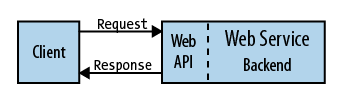
\includegraphics[width=7cm]{figuras/rest_api.eps}
	\caption{\emph{Web API REST}. Fonte: \citeonline{Masse2011}.}
	\label{rest_api}
\end{figure}


Para que um serviço \emph{REST} funcione, ele precisa ser implementado para suportar requisições \emph{HTTP}, ou seja, ele teria que ser um servidor \emph{web} completo. 
A biblioteca escolhida para desempenhar esta função foi a \emph{Flask}. 
Esta é uma biblioteca escrita na linguagem \emph{Python} e fornece todos as ferramentas necessárias para criar aplicações \emph{webs}. 
Segundo \citeonline{Maia2015}, o \emph{Flask} vem sendo adotado, por sua filosofia minimalista que não impõe uma arquitetura específica de projeto, assim permitindo que um projeto comece pequeno e simples, evoluindo para um modelo mais complexo.


\subsection{SERVIÇO DE BASE DE DOCUMENTOS COM \emph{MONGODB}}
\label{mongodb_sec}

Conforme \citeonline{Chodorow2013}, o \emph{MongoDB} é poderoso, flexível e um banco de dados de propósito geral bastante escalável. Ele combina a habilidade de alta escalabilidade com índices secundários, pesquisas limitadas, ordenamento, agregações e índices geoespaciais.

O \emph{MongoDB} é classificado como um banco \emph{NoSQL}. Segundo \citeonline{Dayley2014}, o conceito de \emph{NoSQL} consiste em tecnologias que provêm armazenamento e recuperação sem o amarrado modelo tradicional de bancos de dados Relacionais. A motivação para estas tecnologias é o design simplificado, escalabilidade horizontal e controle fino na disponibilidade dos dados.

O \emph{MongoDB} como toda grande ferramenta de software, foi designado baseado em filosofias próprias, que para os novatos, às vezes pode parecer um contrassenso. 
\citeonline{Plugge2014} comenta que o pináculo das filosofias do \emph{MongoDB} é a noção de que um tamanha não se adéqua a todos. Por muitos anos bancos de dados relacionais foram usados para armazenar conteúdos de todos os tipos. O principal motivo para isso é que ler e escrever em bancos de dados relacionais é muito mais seguro do que fazer o mesmo em arquivos de sistema operacional.
É comum no uso de bancos de dados relacionais, ter que se criar dezenas de tabelas para se armazenar dados complexos, e ainda tentar fazer todas funcionarem juntas.

Ainda, segundo \citeonline{Plugge2014}, a equipe do \emph{MongoDB} decidiu que não ia criar outro banco de dados para resolver todos os problemas do mundo. Eles criaram um banco que trabalha com documentos ao invés de linhas em tabelas. Essa decisão tornou o \emph{MongoDB} muito rápido, altamente escalável e fácil de usar. Por exemplo, o \emph{MongoDB} não suporta transações, logo você não irá escrever uma aplicação de conta corrente com ele. Sua força está armazenar dados muito complexos. No final o desenvolvedor ainda tem a opção de usar um banco de dados relacional que suporta transação e as vantagens do \emph{MongoDB} para outras partes da aplicação, que se aproveitarão melhor do modelo de documentos.


A Figura \ref{mongodb} mostra como os dados são organizados nesta tecnologia.

\begin{figure}[ht]
	\centering
	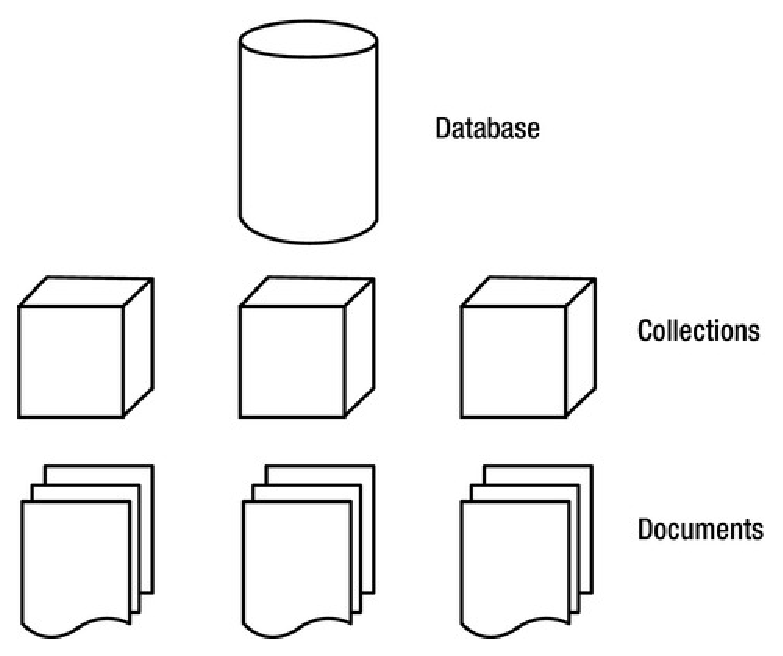
\includegraphics[width=10cm]{figuras/mongodb.eps}
	\caption{Organização dos dados no \emph{MongoDB}. Fonte: \citeonline{Plugge2014}.}
	\label{mongodb}
\end{figure}

Segundo a Figura \ref{mongodb}, um banco de dados \emph{MongoDB} é composto por coleções de dados. 
Dentro destas coleções existem documentos. 
Os documentos dentro de uma coleção não precisam ser do mesmo tipo. 
Mas esta é uma prática pouco recomendada \cite{Plugge2014}. 
Os documentos são armazenados no formato \emph{Binary Object Notation (BSON)}, um primo muito próximo do \emph{JavaScript Object Notation (JSON)}. 
O \emph{BSON} é muito parecido com o \emph{JSON}. Ele foi criado para ser mais otimizado nas leituras e escritas no banco. A Figura \ref{listagem1} retirada de \citeonline{Dayley2014}, mostra como um documento se parece.

\begin{figure}[H]
	\centering
	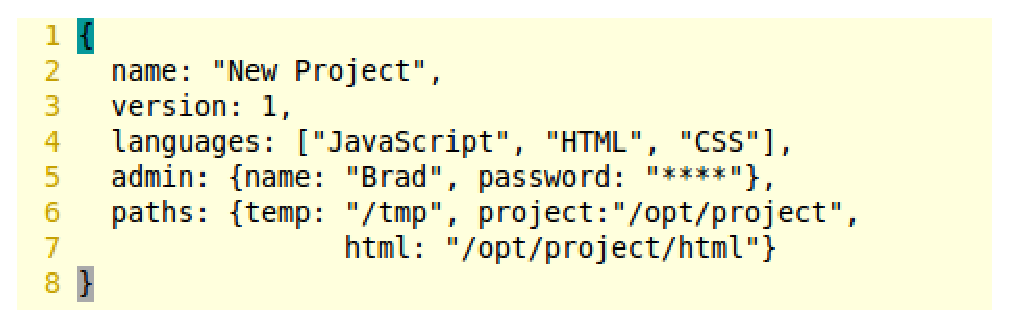
\includegraphics[width=12cm]{figuras/listagem1.eps}
	\caption{Listagem de um documento. Fonte: \citeonline{Dayley2014}.}
	\label{listagem1}
\end{figure}


Para quem conhece \emph{JSON}, provavelmente compreendeu todo o documento. Um documento fica entre \{\} e pode conter outros documentos, tipos simples e listas.
O documento possui atributos, no exemplo, \emph{name, version, languages, admin, paths}. Os atributos \emph{name version} são atributos de tipos simples, texto e número no caso. O atributo \emph{languages} é uma lista e os demais são outros objetos.

A questão da normalização dos objetos é sempre uma decisão do desenvolvedor. É perfeitamente possível tratar coleções e documentos, como tabelas. Como cada tabela tem um identificador único gerado pelo sistema é possível inclusive fazer referência entre documentos. Mas o ideal é encontra um meio termo, onde dados muito acessados juntamente, fiquem numa estrutura hierárquica como a da listagem acima \cite{Dayley2014}. A Figura \ref{normalizacao} mostra como se pode fazer a referência entre documentos.

\begin{figure}[ht]
	\centering
	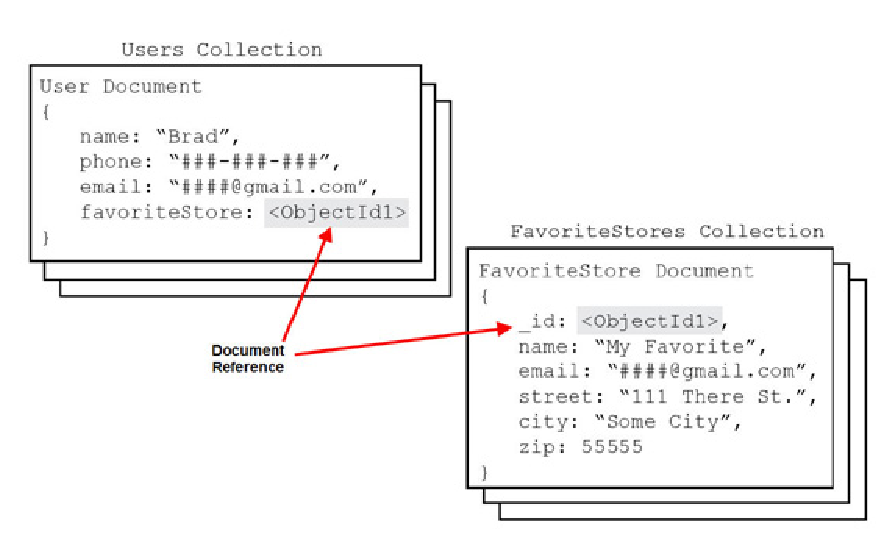
\includegraphics[width=12cm]{figuras/normalizacao.eps}
	\caption{Definindo documentos normalizado com \emph{MongoDB}. Fonte: \citeonline{Dayley2014}.}
	\label{normalizacao}
\end{figure}
